\chapter{$B_{tag}$ fit}

The normalization for the branching fractions is determined from the number of correctly tagged $B$ mesons. 
This value is again determined by fitting the $M_{bc}$ distribution of all $B$ meson candidates tagged
by FEI regardless of the signal side $B$ meson decay.\\
The tagged $B$ meson candidates are selected according to the selection criteria used for the $M_{bc}$ variable  
already illustrated in subsections \crefrange{sec:chargedCorrBtoLambdaC}{sec:neutralAcorrBtoLambdaC}.

%!!! here tell that the Btag samples are selected with same selections as given in selection.tex file. 
% \ref{sec:chargedCorrBtoLambdaC}

\section{Probability Density Functions (PDFs) for the $B_{tag}$}

The reconstructed events can be categorized as follows:
\begin{itemize}
    \item correctly reconstructed $B$ meson candidates: \textbf{reconstructed signal} 
    \item misreconstructed $B$ meson candidates: \textbf{misreconstructed signal}
    \item $B^0$ mesons misreconstructed as $B^+$ (and vice-versa): \textbf{crossfed background} 
    \item and \textbf{continuum background}
\end{itemize}

\subsection{Total Signal fits}\label{sigBtagFit}

As in the 2D fits the total signal is distinguished in \textbf{reconstructed}  and \textbf{misreconstructed signal} depending
on wether it's peaking or not in  $M_{bc}$.\\
\cref{fig:chargedBtag_corrLambdaC_TotalSignalBtag_fit} shows the fit on tagged charged $B$ mesons corresponding to the normalization for the branching fractions of $B^- \rightarrow \Lambda_c^+$ decays.
The $M_{bc}$ distribution of the tagged  $B$ mesons is fitted with a combination of Crystal Ball and Gaussian as for the "peaking" component and the "flat" component is fitted with a Novosibirsk function. 
For the other decay channels instead an Argus function is used to describe the misreconstructed signal (see \crefrange{fig:anticorr_chargedBtag_Total_Signal_fit}{fig:stream0_neutralBtag_anticorrLambdaC_TotalSignal_addedGaussian}).
%Fits show pulls exceeding 3$\sigma$ deviation in some regions, especially in the endpoint region.
%Therefore, in the final fits, the range will be restricted to avoid possible systematic effetcs in the endpoint region.

\begin{figure}[H]
\centering
{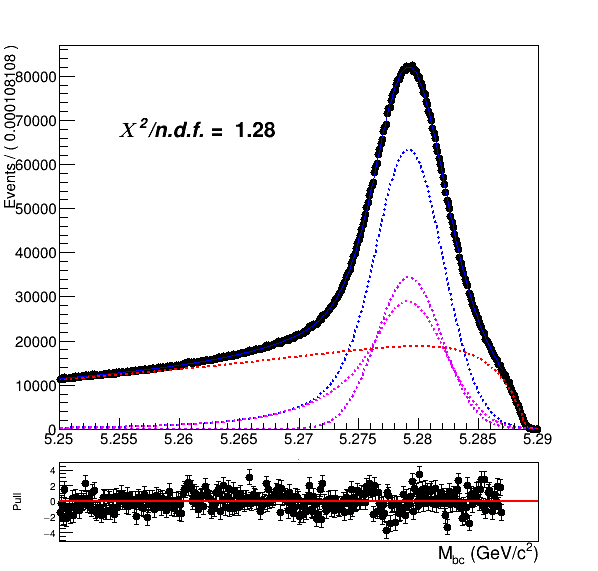
\includegraphics[width=0.40\textwidth]{05-BtagFit/figs/chargedBtag_corrLambdaC_TotalSignalBtag_fit.png}}
\caption{Fitted distribution of tagged charged $B$ mesons in the charged correlated decays sample: reconstructed signal events are described by the blue dotted PDF, the misreconstructed with a Novosibirsk function (red dotted). }
\label{fig:chargedBtag_corrLambdaC_TotalSignalBtag_fit}
\end{figure}

\begin{figure}[H]
    \centering
    {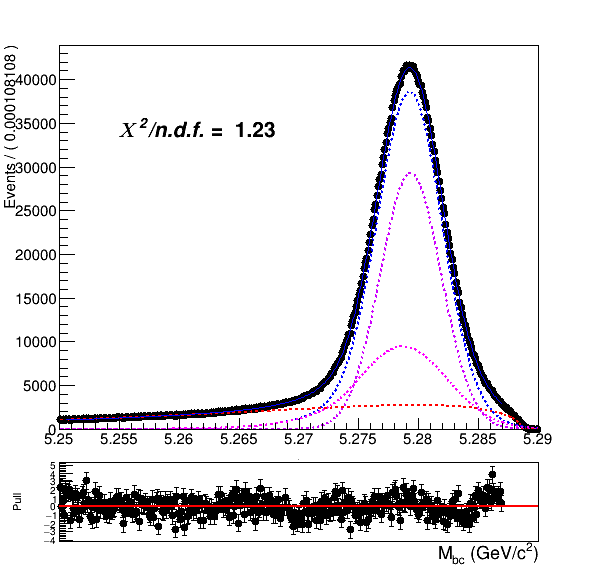
\includegraphics[width=0.40\textwidth]{05-BtagFit/figs/stream1_anticorr_chargedBtag_Total_Signal_fit.png}}
    \caption{Fitted distribution of tagged charged $B$ mesons  in the charged anticorrelated decays sample. }
    \label{fig:anticorr_chargedBtag_Total_Signal_fit}
    \end{figure}

\begin{figure}[H]
\centering
{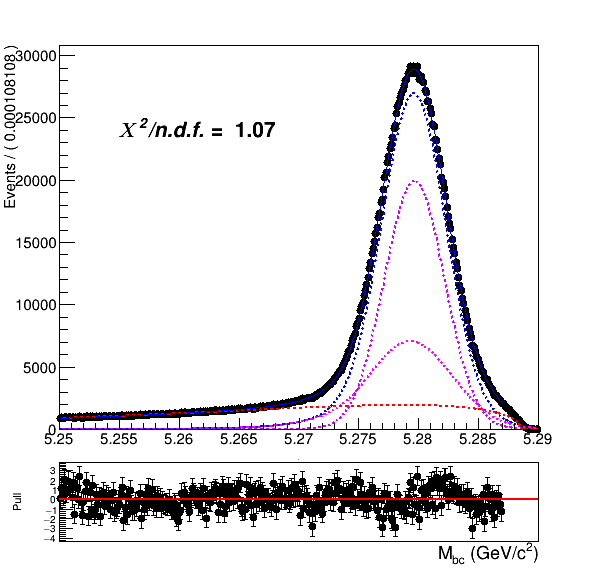
\includegraphics[width=0.40\textwidth]{05-BtagFit/figs/stream0_neutralBtag_corrLambdaC_TotalSignal_addedGaussian.png}}
\caption{Fitted distribution of tagged neutral $B$ mesons reconstructed in neutral correlated decays. }
\label{fig:stream0_neutralBtag_corrLambdaC_TotalSignal_addedGaussian}
\end{figure}

\begin{figure}[H]
\centering
{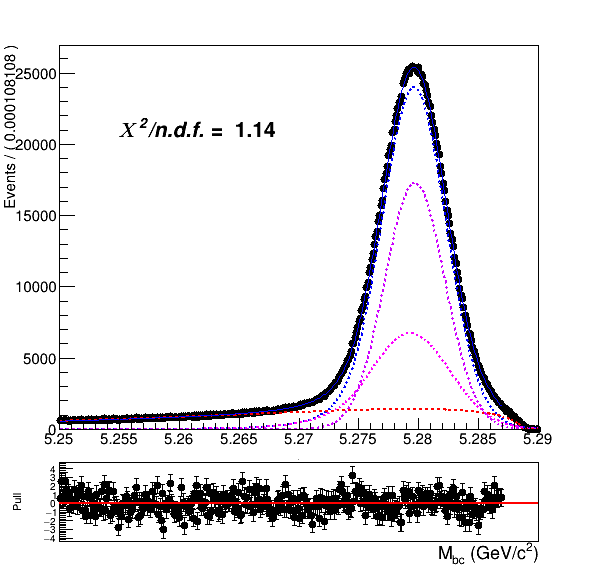
\includegraphics[width=0.40\textwidth]{05-BtagFit/figs/stream0_neutralBtag_anticorrLambdaC_TotalSignal_addedGaussian.png}}
\caption{Fitted distribution of tagged charged $B$ mesons reconstructed in neutral anticorrelated decays. }
\label{fig:stream0_neutralBtag_anticorrLambdaC_TotalSignal_addedGaussian}
\end{figure}
                        

\subsection{Crossfeed PDF}
 
The crossfeed background is always fitted instead with a sum of a Novosibirsk and an asymmetric Gaussian PDF. 

\begin{figure}[h!]
\centering
{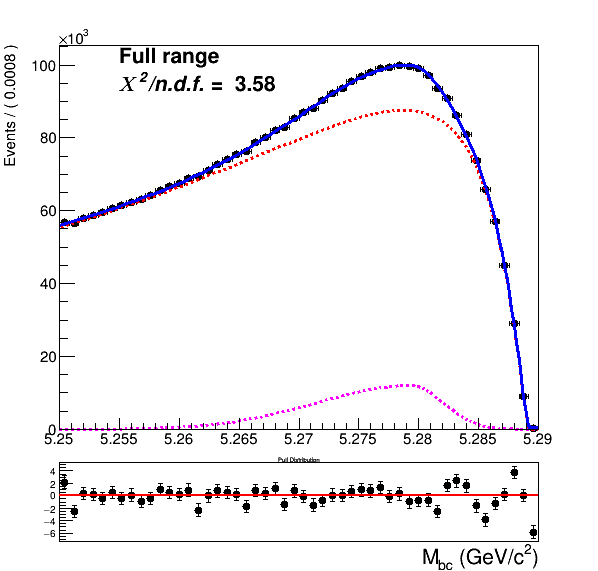
\includegraphics[width=0.40\textwidth]{05-BtagFit/figs/NeutralCrossfeed_stream0_corrLambdaC_chargedBtagFit.png}}
\caption{Crossfeed distribution of charged correlated decays fitted with a sum of Novosibirsk (red) and asymmetric Gaussian PDF (magenta)}
\label{fig:NeutralCrossfeed_stream0_corrLambdaC_chargedBtagFit}
\end{figure}

\begin{figure}[h!]
\centering
{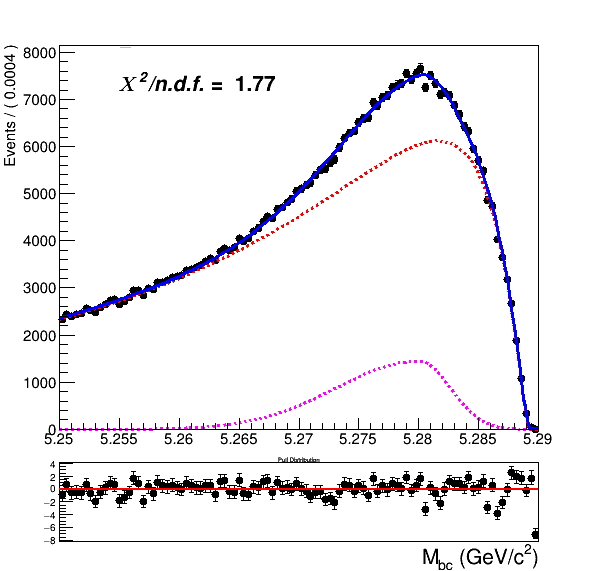
\includegraphics[width=0.40\textwidth]{05-BtagFit/figs/NeutralCrossfeed_stream0_anticorrLambdaC_chargedBtag_MbcFit.png}}
\caption{Crossfeed distribution of charged anticorrelated decays}
\label{fig:NeutralCrossfeed_stream0_corrLambdaC_chargedBtagFit}
\end{figure}

\newpage

\begin{figure}[H]
\centering
{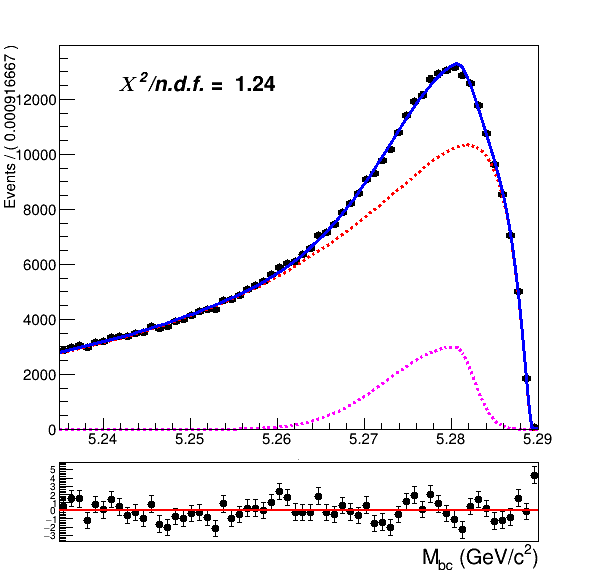
\includegraphics[width=0.40\textwidth]{05-BtagFit/figs/ChargedCrossfeed_stream0_corrLambdaC_neutalBtag_MbcFit.png}}
\caption{Crossfeed distribution of neutral correlated decays}
\label{fig:ChargedCrossfeed_stream0_corrLambdaC_neutalBtag_MbcFit}
\end{figure}

\begin{figure}[H]
\centering
{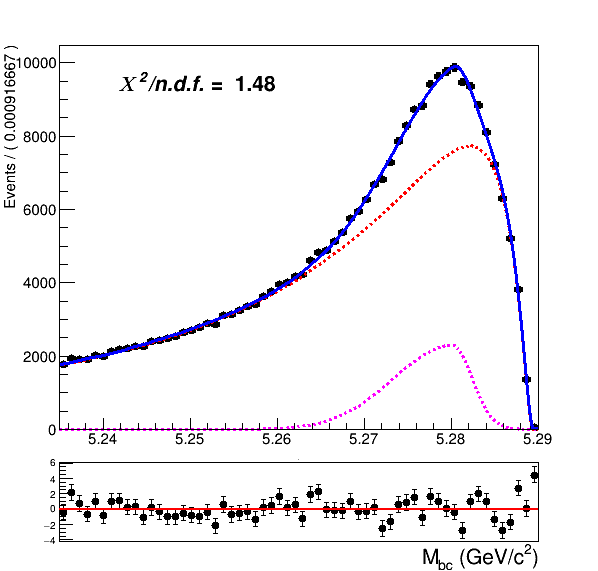
\includegraphics[width=0.40\textwidth]{05-BtagFit/figs/ChargedCrossfeed_stream0_anticorrLambdaC_neutralBtag_MbcFit.png}}
\caption{Crossfeed distribution  of neutral anticorrelated decays}
\label{fig:ChargedCrossfeed_stream0_anticorrLambdaC_neutralBtag_MbcFit}
\end{figure}

\newpage

\subsection{Continuum PDF}
\noindent  As for the continuum background, a similar procedure as the one described already for the two dimensional fit was adopted:

\begin{itemize}
    \item first the off-resonance sample is scaled accordingly
    \item the ratio between the scaled off-resonance and the on-resonance in MC is calculated in each bin (see Fig.\ref{fig:stream0_chargedBtag_off-on_resonance_correct})
    \item the bin-correction is applied on an independent stream and the scaled and bin-corrected $M_{bc}$ distribution is compared with the on-resonance distribution as shown in Fig.\ref{fig:bin_corrected_stream1_off-resonance_on_stream0_on-resonance}
\end{itemize}
\vspace{0.5cm}
Being the statistics much larger than in the 2D sample, there's no need to remove the continuum suppression cut on the off-resonance sample. 

\begin{figure}[H]
 \centering
\subcaptionbox{\label{fig:stream0_chargedBtag_off-on_resonance_correct}}
{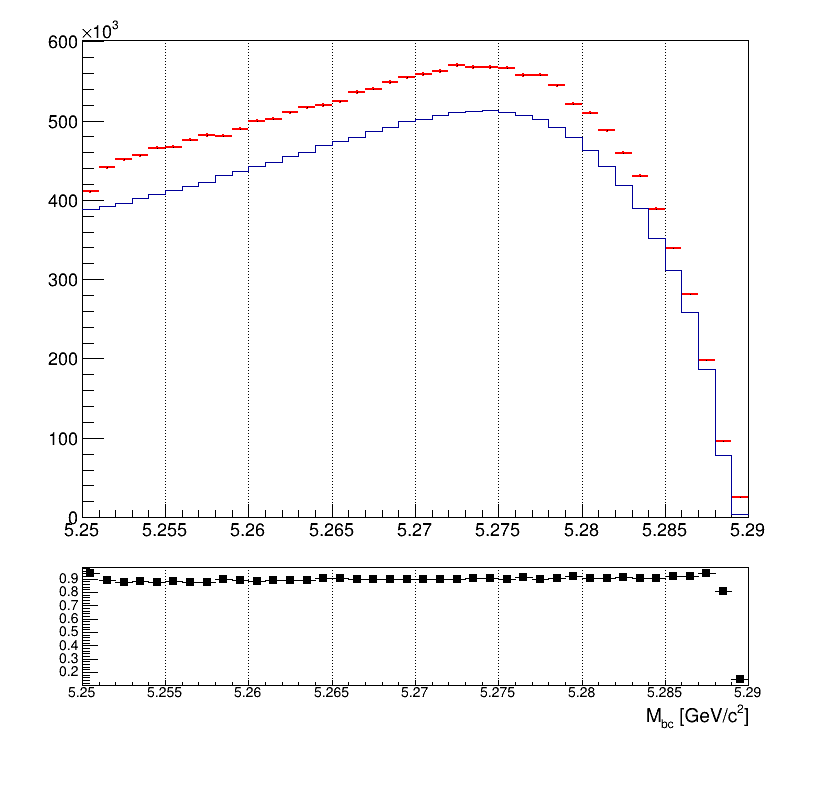
\includegraphics[width=.45\textwidth]{05-BtagFit/figs/stream0_chargedBtag_off-on_resonance_correct.png}}
\subcaptionbox{\label{fig:bin_corrected_stream1_off-resonance_on_stream0_on-resonance}}
{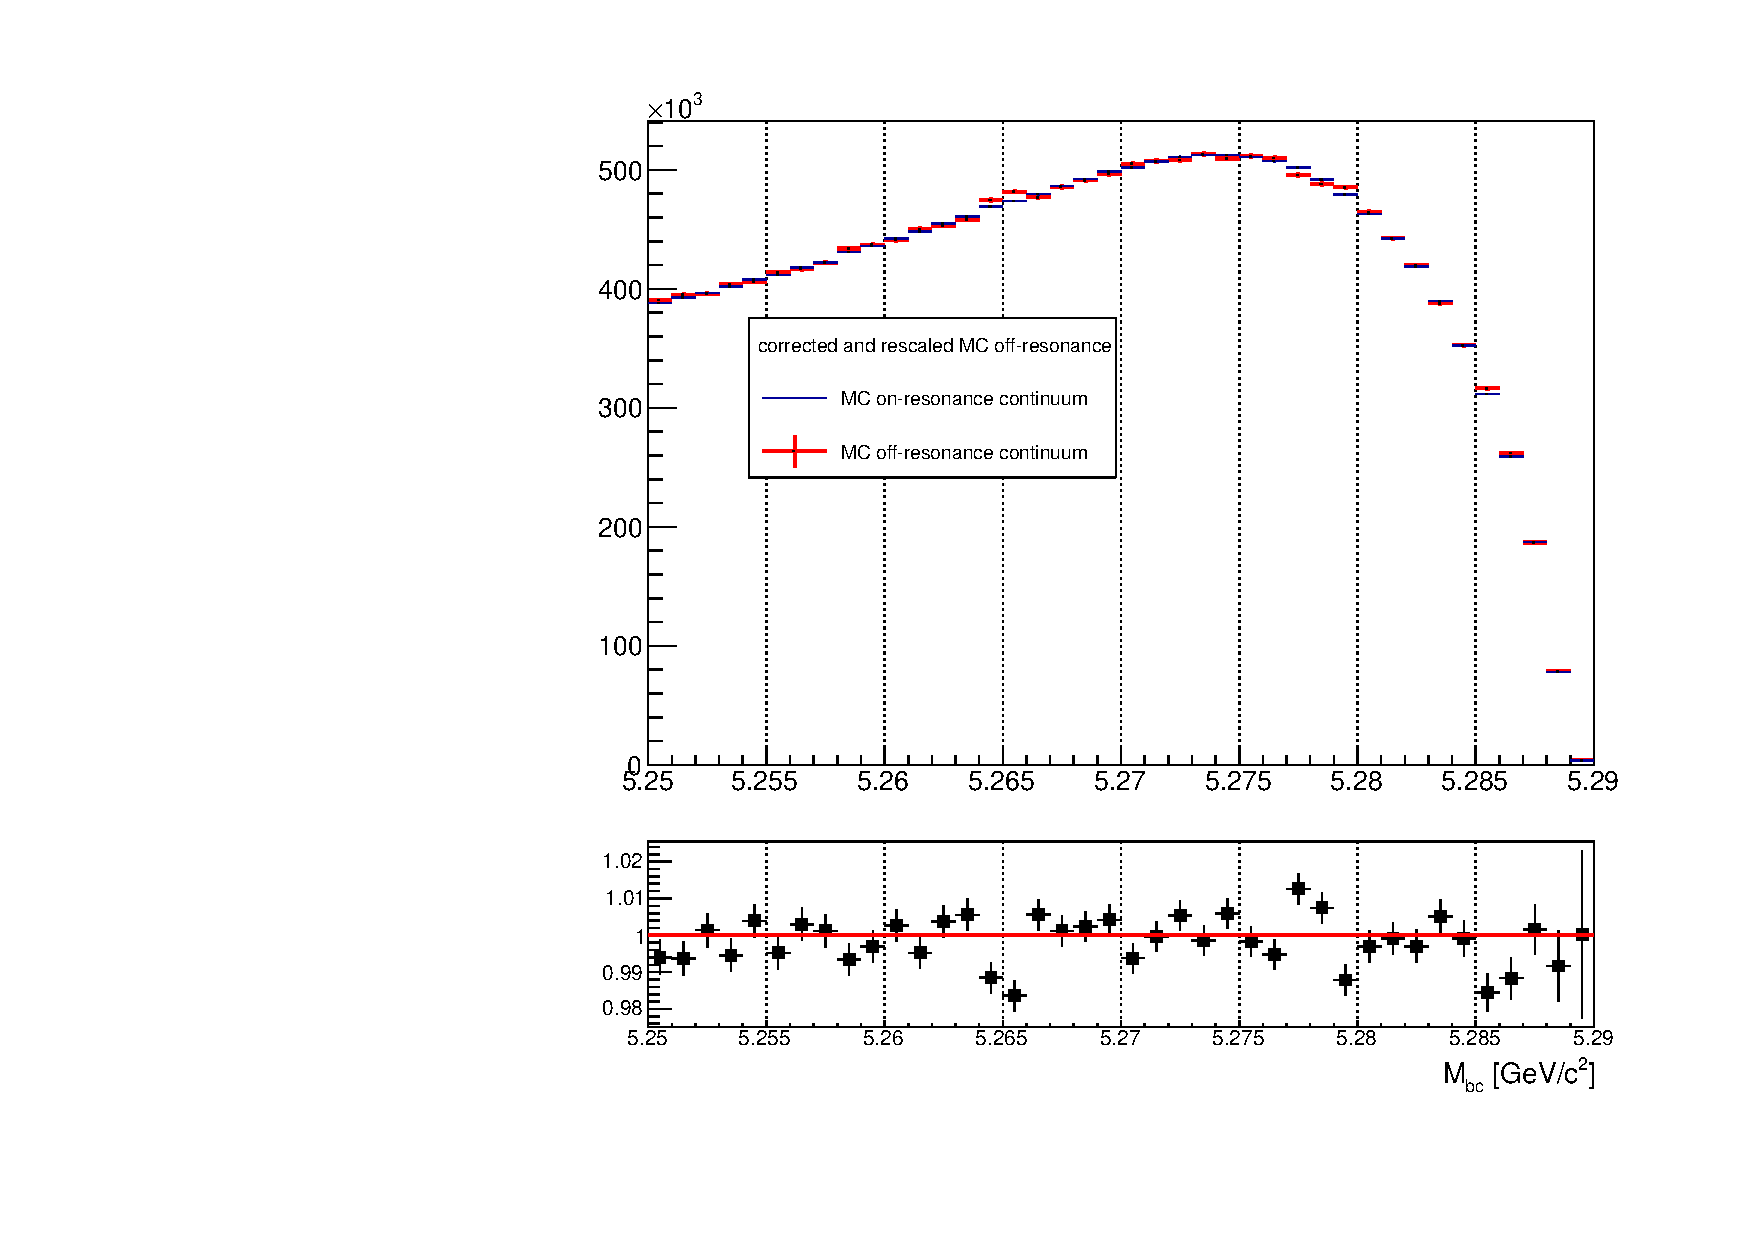
\includegraphics[width=.45\textwidth]{05-BtagFit/figs/bin_corrected_stream1_off-resonance_on_stream0_on-resonance.pdf}} 
\caption{On the left: $M_{bc}$ distributions of the MC off-resonance sample and the MC continuum sample with applied continuum suppression. On the right: $M_{bc}$ distributions of the corrected scaled MC off-resonance and on-resonance MC continuum.}
\end{figure}



\newpage
\section{ $B_{tag}$ fit}\label{BtagFit_onMC}
An independent Monte Carlo stream was used to test the total fit model on tagged $B$ meson candidates.
As in the 2D fit, the parameter for the width, $\sigma_{CB}$, of the Crystal Ball is floated. 
The ratio between expected crossfeed background events and  misreconstructed signal events is fixed from the MC. 
The misreconstructed signal PDF is also not fully constrained: the parameter describing the tail is free. 
To avoid introducing significant systematic uncertainties in the fit deriving from the $M_{bc}$ endpoint region, where one has a smearing effect due to variations of the
beam energy at the MeV level, the range for the fit is restricted to values betweeen 5.250 and 5.287 GeV/c$^2$.


\subsection{Fit results for $B^- \rightarrow \Lambda_c^+$ decays}  


\begin{figure}[H]
    \centering
    {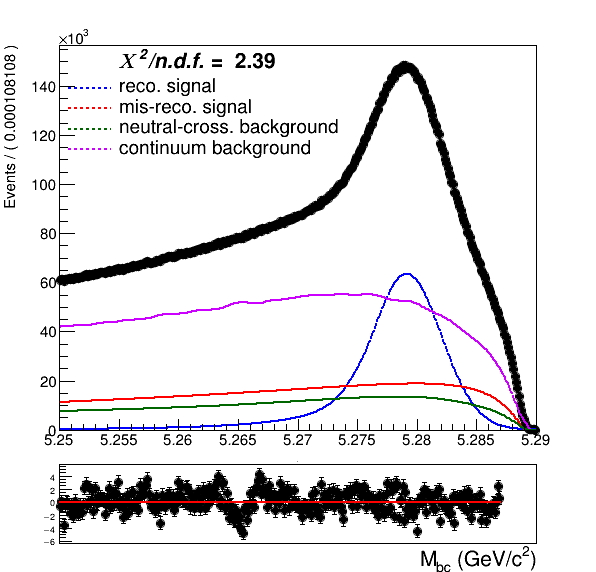
\includegraphics[width=0.50\textwidth]{05-BtagFit/figs/NEW_stream5_chargedBtag_Total_fit_sigmaCB_misReco_Tail_free_370bins.png}}
    \caption{Total fit of tagged $B$ mesons on Monte Carlo simulated data.}
    \label{fig:chargedCorrLambdaC_BtagFit}
    \end{figure}
    \vspace{1.5cm} 

Yields for the reconstructed and misreconstructed signal are obtained from the fit:\\
\vspace{0.25 cm}

\begin{tabular}{ |p{2.5cm}||p{4.2cm}| p{4.2cm}|  }
 \hline
          &    Fit results                 &  expected\\
 \hline
 NrecSig  & 4.7787 $\cdot$10 $^6 \pm$ 6748 &  4.7571 $\cdot$10 $^6 \pm$ 3214 \\
 NmisSig &  5.3987 $\cdot$10 $^6 \pm$ 5617 & 5.4035 $\cdot$10 $^6 \pm$ 3376 \\
 \hline
\end{tabular}

\vspace{0.5 cm}
The normalization for the branching fraction is given by the NrecSig yields. The yields obtained in the fit differ by $\sim 3.2 \sigma$ 
from the expected ones (obtained from a fit to the Total Signal events only).  This discrepancy will impact the final 
measurement.

%The Total Signal (the sum  NrecSig+NmisSig) is 10134027 $\pm$ 4402 (to be compared with 10157950 from the Monte Carlo). 
% This reflects a $\sim 5.5\sigma$ discrepancy between the true MC value and the result from the fit. This can produce some systematic effect, 
 %but the relative error is at the $\sim$ \textperthousand level. 
 %This is still negligible compared to the systematic uncertainity corresponding to the the ${N_{tag}}$ determination, 
 %and furthermore in the branching fraction calculation it is also negligible compared to the statistical uncertainity on 
 %the extracted yields 
%from the two dimensional fit.
 
To check the stability of the fit model a toy MC study was performed with  $3\times10^3$ pseudo-datasets. 
No evidence for possible biases in the reconstructed signal yields was found (see \cref{fig:NrecSignalchargedCorrBtag_mcstudy}).


\begin{figure}[H]
    \centering
    {\centering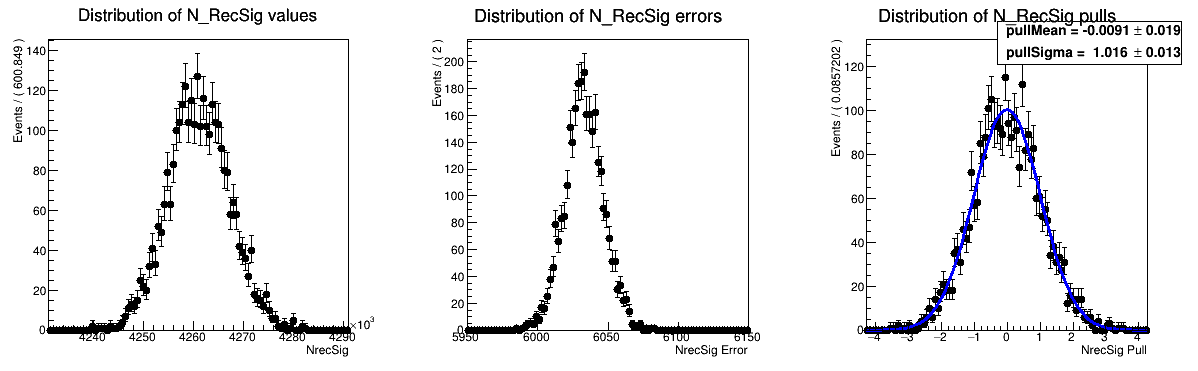
\includegraphics[width=14cm]{05-BtagFit/figs/NrecSigBtag_mcstudy.png}}
     \caption{Plots showing distributions of the fitted signal yields, errors and the pull distribution of
    all pseudo-fits. (see Appendix \ref{sec:chargedBtoLamApp} for the other free parameters' results)}
      \label{fig:NrecSignalchargedCorrBtag_mcstudy}
      \end{figure}



\subsection{Fit results for $B^- \rightarrow \bar{\Lambda}_c^-$ decays}  
\begin{figure}[H]
    \centering
    {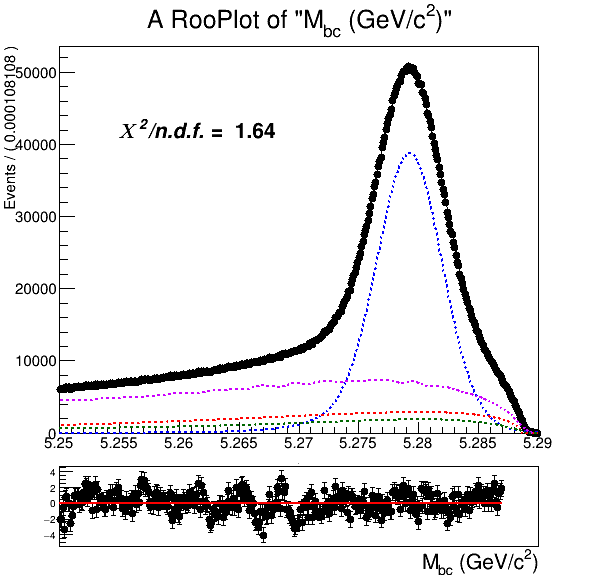
\includegraphics[width=0.50\textwidth]{05-BtagFit/figs/NEW_chargedBtag_anticorrLambdaC_Total_fit_sigmaCB_misRecoSlope_free_370bins.png}}
    \caption{Total fit of tagged $B$ mesons on Monte Carlo simulated data.}
    \label{fig:chargedAntiLambdaC_BtagFit}
    \end{figure}
    \vspace{1.5cm} 


    \begin{tabular}{ |p{2.5cm}||p{4.2cm}|  }
        \hline
        NrecSig  & 2.50831$\cdot$10$^6 \pm$ 11866\\
        NmisSig &  7.37010$\cdot$10$^5 \pm$ 7472 \\
        \hline
       \end{tabular}
       
       
       \vspace{0.5 cm}
       \noindent The Total Signal (the sum  NrecSig+NmisSig) is 3292168 $\pm$ 2423 (to be compared with 3299629 from the Monte Carlo), which means a $\sim 3\sigma$ underestimation. As in the case of charged flavor-correlated decays, this can produce some systematic effect which needs to be taken into account.
       %In fact, a slight underestimation of the Total Signal is found also in the result of the toy Monte Carlo study: \cref{fig:Total_Signal_chargedBtagToyMCstudy} shows the results for the Total Signal events and one can notice a mean value for the pulls consistently below zero.
       
%\begin{figure}[H]
      %  \centering
      %  {\centering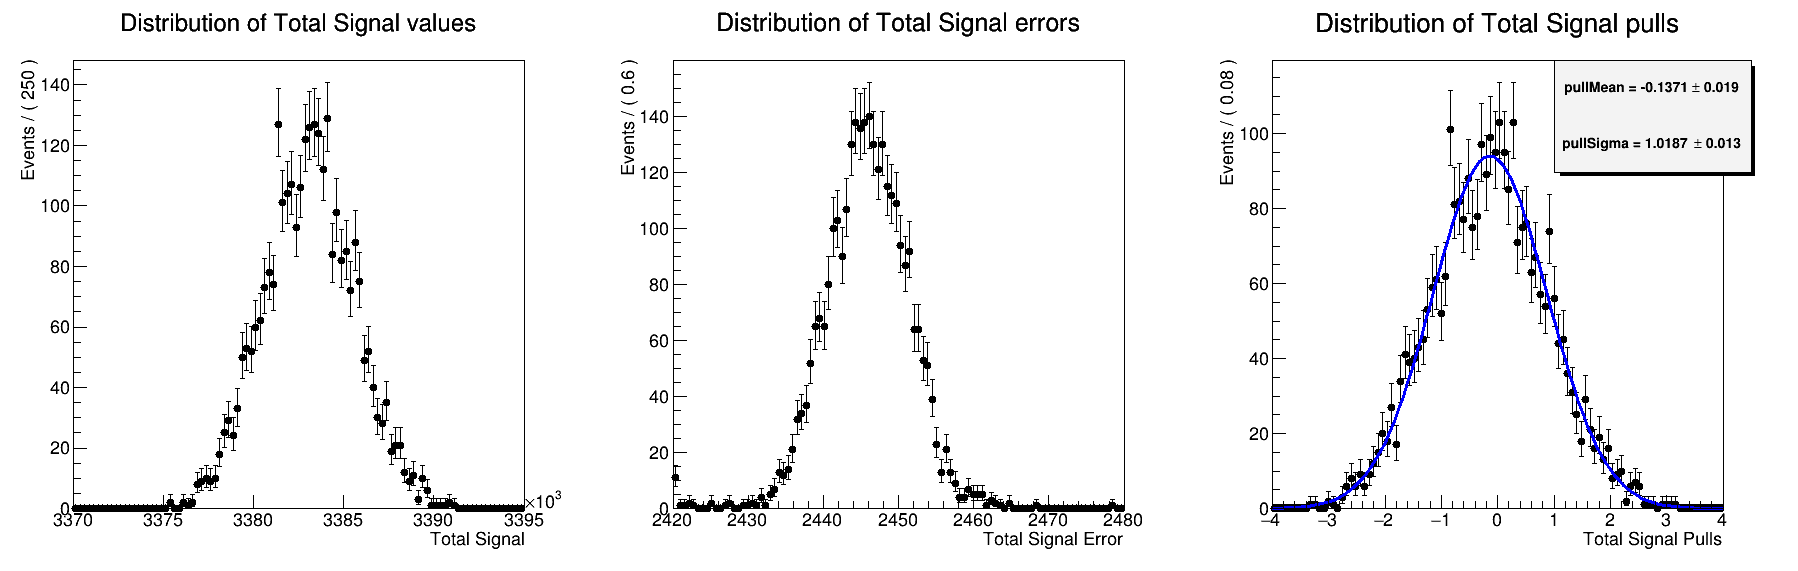
\includegraphics[width=14cm]{05-BtagFit/figs/Total_Signal_chargedBtagToyMCstudy.png}}
%\caption{Plots showing distributions of the fitted signal yields, errors and the pull distribution of
     %   all pseudo-fits. (see Appendix \ref{sec:chargedBtoLamApp} for the other free parameters' results)}
     %     \label{fig:Total_Signal_chargedAntiBtagToyMCstudy}
     %     \end{figure}
       
But when performing a toy Monte Carlo study\footnote{as usual performed with  $3\times10^3$ pseudo-datasets} 
the result show no bias on the recosntructed signal yields (see \cref{fig:NrecSig_chargedAntiBtag_mcstudy})


\begin{figure}[H]
    \centering
    {\centering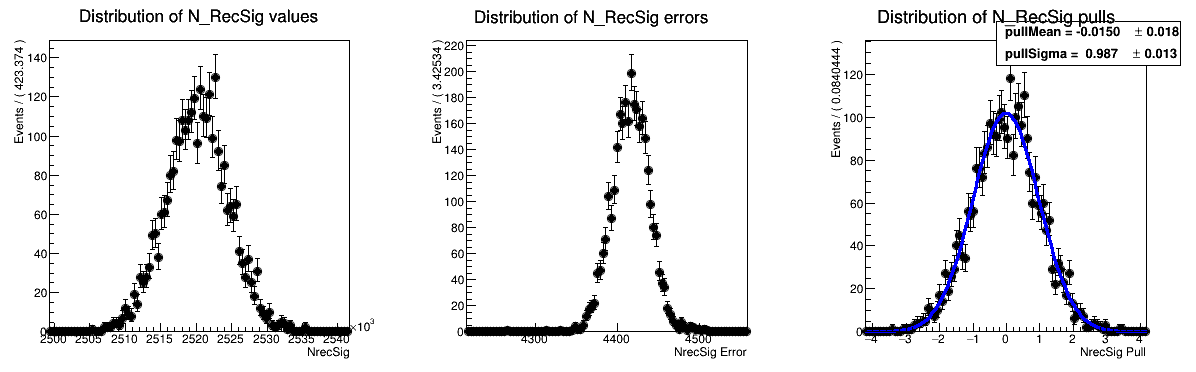
\includegraphics[width=14cm]{05-BtagFit/figs/NrecSig_chargedAntiBtag_mcstudy.png}}
    \caption{Plots showing distributions of the fitted signal yields, errors and the pull distribution of
    all pseudo-fits. }
    \label{fig:NrecSig_chargedAntiBtag_mcstudy}
    \end{figure}
                     


\subsection{Fit results for $\bar{B^0} \rightarrow \Lambda_c^+$ decays} 

\begin{figure}[H]
    \centering
    {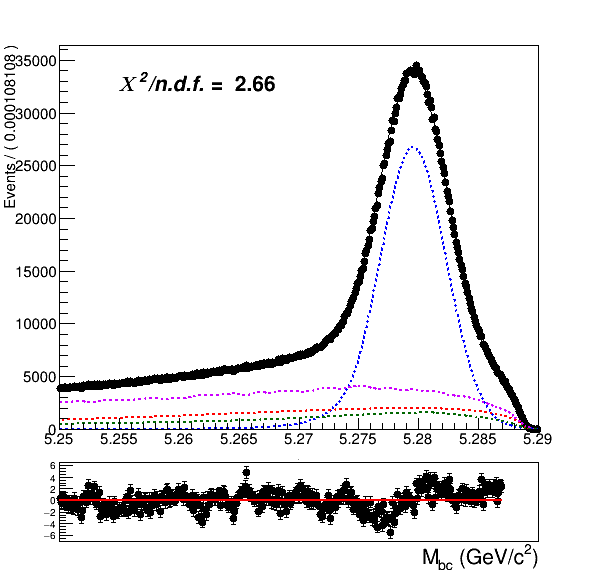
\includegraphics[width=0.50\textwidth]{05-BtagFit/figs/neutralCorrLambdaC_BtagFit.png}}
    \caption{Total fit of tagged $B$ mesons on Monte Carlo simulated data.}
    \label{fig:neutralCorrLambdaC_BtagFit}
    \end{figure}
    \vspace{1.5cm} 

Reconstructed and misreconstructed signal yields obtained from the fit:\\
    \vspace{0.25 cm}
    
    \begin{tabular}{ |p{2.5cm}||p{4.2cm}|  }
     \hline
     NrecSig  & 1.7215 $\cdot$10 $^6 \pm$ 3421\\
     NmisSig &  5.5950 $\cdot$10 $^5 \pm$ 2215 \\
     \hline
    \end{tabular}      
    
    \vspace{0.5 cm}
    \noindent The Total Signal (the sum  NrecSig+NmisSig) is 2281033 $\pm$ 1947 (to be compared with 2286964 from the Monte Carlo).
    Also in this case there's a $\sim 3\sigma$ underestimation. 
   
 \vspace{0.5 cm}
       
\begin{figure}[H]
\centering
{\centering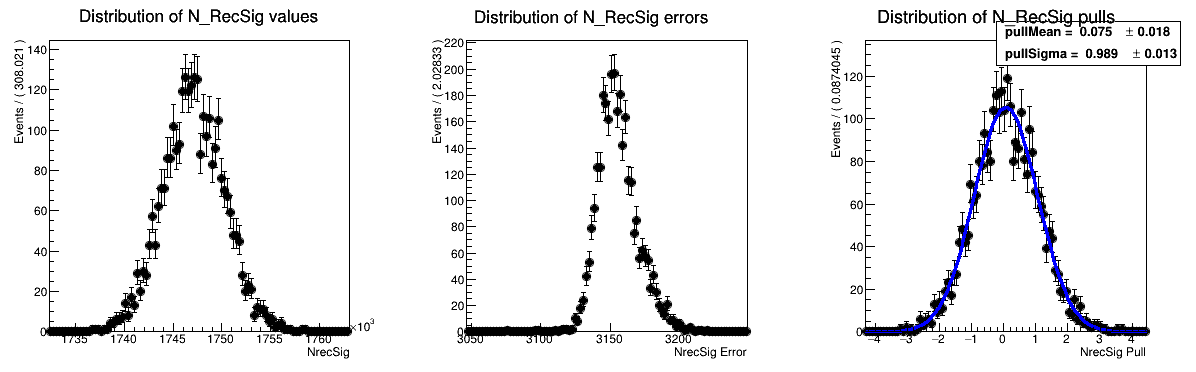
\includegraphics[width=14cm]{05-BtagFit/figs/NrecSig_neutralCorrBtag_mcstudy.png}}
\caption{Plots showing distributions of the fitted signal yields, errors and the pull distribution of
all pseudo-fits. }
\label{fig:NrecSig_neutralCorrBtag_mcstudy}
\end{figure}
       

    

\subsection{Fit results for $B^0 \rightarrow \bar{\Lambda}_c^+$ decays} 



\begin{figure}[H]
    \centering
    {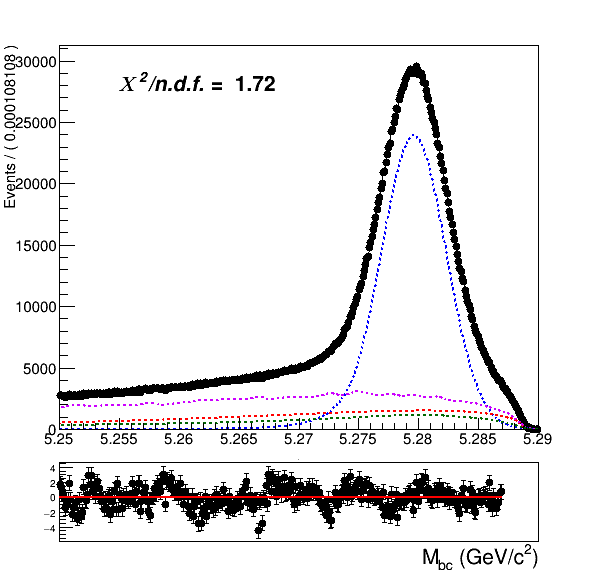
\includegraphics[width=0.50\textwidth]{05-BtagFit/figs/stream1_neutralBtag_Total_fit_sigmaCB_misReco_slope_free_370bins.png}}
    \caption{Total fit of tagged $B$ mesons on Monte Carlo simulated data.}
    \label{fig:neutralAntiLambdaC_BtagFit}
    \end{figure}
    \vspace{1.5cm} 

Reconstructed and misreconstructed signal yields obtained from the fit:\\
    \vspace{0.25 cm}
    
    \begin{tabular}{ |p{2.5cm}||p{4.2cm}|  }
     \hline
     NrecSig  & 1.5302 $\cdot$10 $^6 \pm$ 3269\\
     NmisSig &  3.8332 $\cdot$10 $^5 \pm$ 2072 \\
     \hline
    \end{tabular}      
 
   
 \vspace{0.5 cm}
 \noindent The Total Signal (the sum  NrecSig+NmisSig) is 1913476 $\pm$ 1812 (to be compared with 1920156 from the Monte Carlo).
 Also in this case there is an underestimation of about a $\sim 3.7\sigma$. 
 
        
The toy MC study result for the signal yields is shown in \cref{fig:NrecSig_neutralAntiBtag_mcstudy}.
 Also in this case no hints of bias are visible.

\begin{figure}[H]
    \centering
    {\centering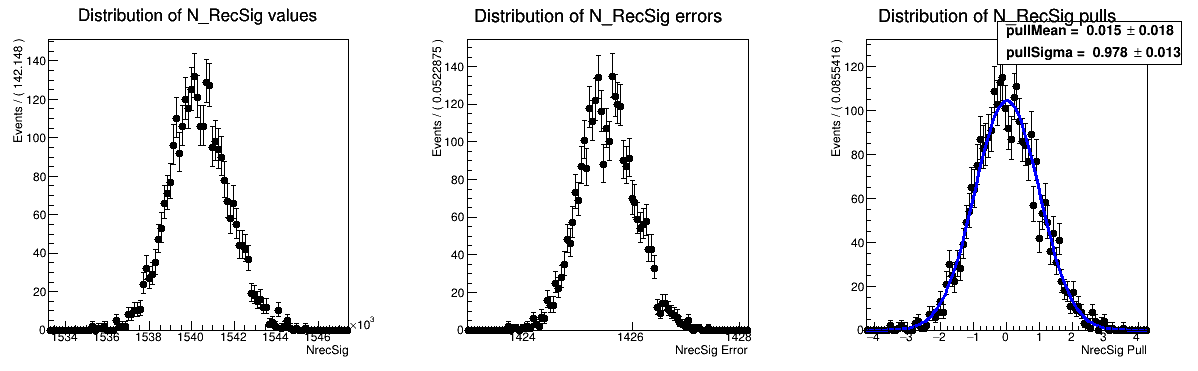
\includegraphics[width=14cm]{05-BtagFit/figs/NrecSigneutralAntiBtag_mcstudy.png}}
    \caption{Plots showing distributions of the fitted signal yields, errors and the pull distribution of
    all pseudo-fits. }
    \label{fig:NrecSig_neutralAntiBtag_mcstudy}
    \end{figure}
